% Chapter Template

\chapter{Reinforcement Learning} % Main chapter title

\label{Chapter4} % Change X to a consecutive number; for referencing this chapter elsewhere, use \cref{ChapterX}


Reinforcement learning (RL) is an area of machine learning concerned with how intelligent agents ought to take actions in an environment in order to maximize the cumulative reward. Reinforcement learning is one of three basic machine learning paradigms, alongside supervised learning and unsupervised learning. \cite{rl} \\

For this project, It was looked for an RL example that is well-documented so it can be customized for the project's needs.
The choice fell on the article "Playing Cards with Reinforcement Learning" \cite{easy21_explanation}, which describes Reinforcement Learning and the principles behind it; also, the Jupyter Notebook is provided \cite{easy21}.
The article uses the game Easy 21 (a variant of BlackJack) to explain the basics of reinforcement learning and three approaches for estimating the best playing strategy. \\

The goal of the following algorithms is to learn the Q value function. The Q value is the estimated potential reward in a given game situation.

%----------------------------------------------------------------------------------------
%	Monte Carlo Control (MCC)
%----------------------------------------------------------------------------------------
\section{Monte Carlo Control (MCC)}
\textbf{Monte-Carlo} means that we are going to play game sequences/episodes (play a round of Jass). The \textbf{Control} part means that we are going to find the optimal policy (best action to pick to maximize our winning chances). After each round, the Q value gets updated. If the played game was a win (resp. loss), the values of the state-action pair should be increased (resp. decreased)

%----------------------------------------------------------------------------------------
%	SARSA($ \lambda $)
%----------------------------------------------------------------------------------------
\section{SARSA($ \lambda $)}
\textbf{SARSA} is the acronym of State, Action, Revard, State', Action', which is related to the way the algorithm updates the Q value function. The $ \lambda $ is a model's parameter called the trace factor, scaling from 0 to 1. If $ \lambda $=1, we have the classic MCC approach, and if $ \lambda $=0, it is a Temporal-Difference learning update. This means we adjust our current Q value to better match a future Q value estimation.

%----------------------------------------------------------------------------------------
%	Value Approximation (VA)
%----------------------------------------------------------------------------------------
\section{Value Approximation (VA)}
\textbf{Value Approximation} means that we are going to approximate the Q value function rather than computing it for all the possible state-action pairs.

%----------------------------------------------------------------------------------------
%	Adjustments for the JassBot
%----------------------------------------------------------------------------------------
\section{Adjustments for the JassBot}
For the JassBot, some adjustments to the Easy 21 example were necessary. First of all, a "new" game engine (enviroment) had to be written which could interact with the RL algorithms. The number of possible actions was not changed because in Jass (as well as in Easy 21) you can only take two actions (take the trick or not take the trick). The code for the RL algorithms had to be adapted only slightly and could be copied as far as possible from the example.
The value approximation was not pursued further since different typical game situations must be represented. Because of the more than 90 million possible hand combinations, hand coding of significant game situations did not seem purposeful.

% ---------------------------------------------------------------------------------------
\subsection{Game Environment}
The game environment implements the Jass mechanisms. Here the deck of cards and the two players are created. \\
A game lasts until one player has reached 7 points. A game consists of several rounds (also called episodes). A round consists of 9 cards per player (All nine cards in the hand are played). Different functions are implemented (see \ref{agents_actions}) to decide which card to play.

% ---------------------------------------------------------------------------------------
\subsection{Agents and Actions} \label{agents_actions}
The two players are represented by an AGENT, and this agent can choose different functions for selecting a card to play, depending on the situation. \\

For the RL of the first player, two actions are available (take: take the trick or leave: leave the cards on the table/let the other player win the cards). 
\begin{itemize}
    \item take will always play the strongest card possible
    \item leave will always play the weakest card possible
\end{itemize} 

\noindent
For the second player, no RL is used, here the strategy can be defined once in the code, which will always be used (e.g., random, probabilistic, card selection based on the previously learned Q values)
% ---------------------------------------------------------------------------------------
\subsection{Card encoding}
With different encodings, it was examined whether the learning success can be improved if more information is encoded in the numbers. \\
Several methods have been implemented for encoding the cards/game states:
\begin{itemize}
    \item simple: each card has a fixed number (the Trump cards have the highest numbers).
    \item linear numbering: from weak (0) to strong (26)
    \item card strength: Different cards can have the same value
    \item digits1: see Figure \ref{fig:digits1}
    \item digits2: see Figure \ref{fig:digits2}   
\end{itemize}    

\newpage

\begin{figure}[ht!]
    \begin{subfigure}{0.5\textwidth}
        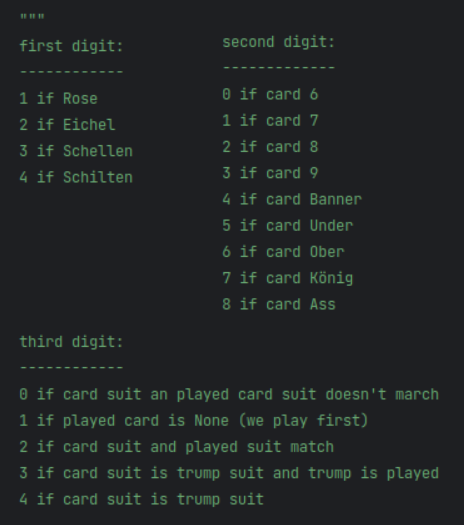
\includegraphics[width=0.9\linewidth]{Figures/digits1} 
        \caption[Digits1]{Digits1}
        \label{fig:digits1}
        \end{subfigure}
        \begin{subfigure}{0.5\textwidth}
        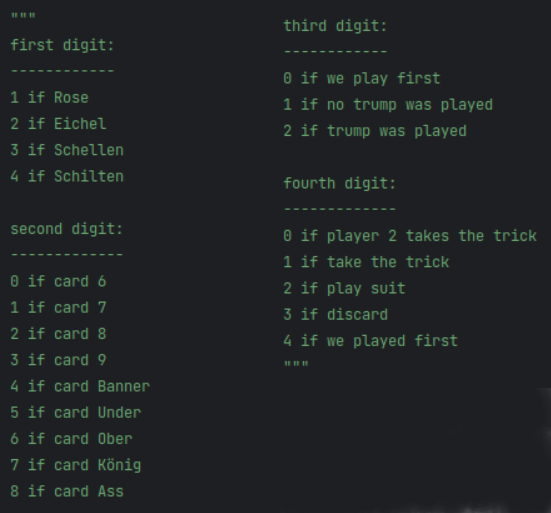
\includegraphics[width=0.9\linewidth]{Figures/digits2}
        \caption[Digits2]{Digits2}
        \label{fig:digits2}
    \end{subfigure}
    \caption{Card encoding}
\label{fig:encoding}
\end{figure}
    

